\chapter{Robotics}
\marginnote{Needs to be refering more to the project requirements}.

This chapter descripes the setup of the robot system used with the focus of making a quick reference for fast setting up a robot system using tool in the ROS framework. The task of the robot in this project is to be able to move the camera sensor around the object to capture images from different poses. For this purpose a 6 axis Stäubli rx60 has been provided along with a ROS service interface to query and control the configuration. The robot and workcell will be descriped in further details in section \ref{sec:robot_physical}. For the robot to be able to move from one pose to another, planners, collision checking and controllers are need. For the planner to be able to do the collision cheking without actually coliding a model of the robot and the workcell must be present. How to setup this model and available parameters are shortly descriped in section \ref{sec:robot_model}. Planning a collision free path is done with ROS MoveIt and ROS Control is used to make the interface between MoveIt and the robot. The MoveIt concepts and how to set it up is descriped in section \ref{sec:moveit}, a further look in to the planning algorihtms in section \ref{sec:planning} and a short introduction to ROS control in section \ref{sec:robot_control}. A graphical overview of the system is given in figure \ref{fig:workcell_to_moveit_path}

\begin{figure}[htb]
	\begin{center}
		
\includegraphics[scale=0.5,trim=0 0 0 0]{graphics/05_robotics/workcell_to_moveIt_path.png}%trim=l b r t
		\caption{Overview of the path from the workcell to the MoveIt stack}
		\label{fig:workcell_to_moveit_path}
	\end{center}
\end{figure}

% Remember to refer the requirement specification, give a breif introduction to why MoveIt has been used and also a short abstact of what this chaper contains.

% General overview of the system

\section{The physical robot and ROS interface}
\label{sec:robot_physical}
% - Staübli (boot up)
The robot provided for this project is a Stäubli RX60b 6 Axis industrial manipulator. When starting the robot a small rotaty switch in the bottom of the controller needs to be turned, and after a few minutes the robot will be booted up and ready. Interfacing the robot is done by a small teach pendant, where it is possible to change application, calibrate, manual control etc. For this project a robot application has been written such that the robot communicated with a ROS node on a provided machine thus almost no interfacing with the robot is nessecary. When starting the robot, it needs to run the robot application which is done by releasing the emergency stop, pushing the big green button i the top right corner so it lids up and pressing the pause button. When doing test with the robot it can be recommended to adjust the moving speed to a minimum to avoid accidents. This is done by the plus and minus buttons on the pendant.
% - The tool unit and sensors (breif)
The tool mounted on the tool flange is a 3D printet sensor mount with both a Carmine depth camera and a PointGrey BumbleBee stereo camera. Wires have been stripped to the robot to avoid them getting stuck in the moving parts. 
% - Workcell
The workcell contains the robot placed on big surface, a troax safety fence and a radiator. Both the fence and the radiator is placed in such distance that the robot will only be able to collide with them in very few configurations. The workcell can be seen in figure \marginnote{Image missing}.

% ------------------------------------------- PICTURE OF ROBOT AND WORKCELL ---------------------------------------

% - The ROS service interface
The robot axis are controlled by the robot controller which are then connected to a computer with a provieded ROS application for communication. To control the robot service calls needs to be made to this node. These service calls provides functionality such as setting various limits, tool position, valve control and most important joint configurations. Furthermore it allows values to be read from the robot, such that feedback to the trajectory controller can be supplied.

\section{Robot model}
\label{sec:robot_model}
To be able to plan a trajectory for the robot, the planner needs a model of the robot. The model is used both for kinematics but also to avoid self collision. The format for descriping a robot in ROS is Unified Robot Description Format (URDF). It is also possible to define the robot in the XACRO format and convert it to the macro language URDF, however in this project the robot has been descriped directly in URDF.
% - URDF format and tools (can also be used in gazebo)
A tool that can be used to generate the URDF file directly from a CAD assembly file is available under the name "SolidWorks to URDF Exporter". This tool was used as a basis for the URDF file for this project, but the quality of the output is somehow questionable. A workcell containing the description of the RX60 robot was available for the project and has been used as a reference to descripe the joints,  joints limits and also source for robot CAD files. It needs to be noticed that CAD format has to be binary STL. The tool of the robot has also been descriped in the URDF to give the nessecary transforms for the camera sensors and a good looking visualization of the robot. In the URDF file it is possible to define both a visual CAD of the joints but also a CAD only used for collision cheking. To be sure that the tool does not collide with anything, the collision model is a large box with a least 10mm extra spacing in respect to the visual model. The model can be seen on figure \ref{fig:tool_collision_model}. To use the URDF file it has to be put into the parameter server which can be done in the launch file \marginnote{Needs explaning?}.

\begin{figure}[htb]
	\begin{center}
		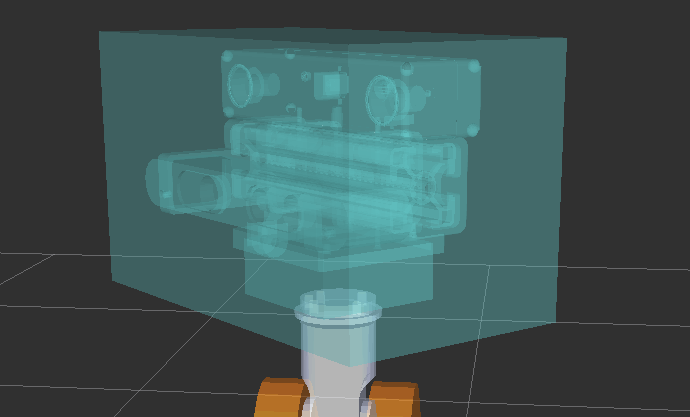
\includegraphics[scale=0.5,trim=0 0 0 0]{graphics/05_robotics/tool_collision_model.png}%trim=l b r t
		\caption{The tool mounted on the robot flange and the collision model shown in transparrent}
		\label{fig:tool_collision_model}
	\end{center}
\end{figure}

% - - Collision model and visual model
% - TF tree
% - Visualization
\section{ROS MoveIt}
\label{sec:moveit}
ROS MoveIt is a software plannig tool that collect many opensource libraries to a tool that can easyly can be used for planning with complex robots. A great example of a complex robot is the PR2 robot developed at Willow Garage that runs on MoveIt.
Controlling a robot with MoveIt can be done by the interface provided in C++ or python but it also features a planning plugin for the ROS visualizer (Rviz). Combining the programming interface with Rviz gives a great visual feedback, where the planned trajectory can be visualized before and while moving the robot as seen on figure \ref{fig:robot_trajectory}.

\begin{figure}[htb]
	\begin{center}
		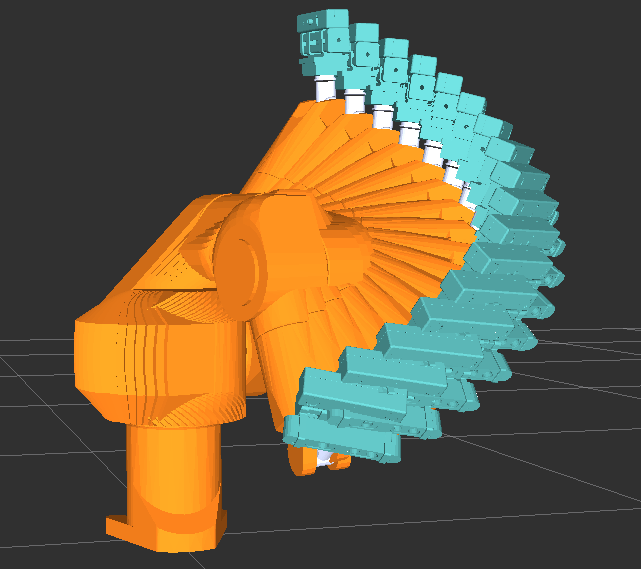
\includegraphics[scale=0.5,trim=0 0 0 0]{graphics/05_robotics/robot_trajectory.png}%trim=l b r t
		\caption{Robot trajectory displayed as a series of poses in Rviz}
		\label{fig:robot_trajectory}
	\end{center}
\end{figure}

% - Features / introduction
% - - Support for octomap input for collsion checking with self-filter (removes visible parts of the robot from the map)
% - - OMPL - Motion planning (OMPL itself has no concept of a robot)
% - - IKFast - Kinematic solver
% - - FCL - Collision checking
% - Importing the robot
% - Interfaces (rviz, c++, trajectory service)
% - - rviz, c++
% - - controller manager (trajectory action interface)
% - Constrainting the robot

% - Robot state publisher (TF)
\section{Planning}
\label{sec:planning}
% - PRM planner
% - Path optimization
% - How is it done in OMPL?
\section{ROS MoveIt}
\section{Robot control}
\label{sec:robot_control}
% - ROS Control framework

%Motion planning
%  general motion planning, kinematics
%  Available tools in ROS
%  MoveIt planner concepts
%  Setting up a new robot with MoveIt
%  Robot model (URDF (joints, links, limits, transforms) , CAD, rviz/TF)
%Robot controller
%
%C++ planning interface
